\documentclass[../../main.tex]{subfiles}
\graphicspath{{images/Maschinentechnik/}{../../images/Maschinentechnik/}}

\lstset{basicstyle=\small,
      showstringspaces=false,
      commentstyle=\color{black},
      keywordstyle=\color{blue}
    }

\begin{document}
    \subsection{Konzeptbeschreibung}
    Die Lokomotive in Abbildung \ref{fig:bg_lokomotive} (siehe Tabelle \ref{tab:bg_lokomotive}) in die drei Unterbaugruppen Antriebswagen (Position 1), Führungswagen (Position 2) und Ladungsträger (Position 3) unterteilt. Der Antriebswagen enthält alle notwendigen Komponenten, um die Lokomotive zu beschleunigen und wieder abzubremsen. Zusätzlich sind die Kameras für die Spur- und Signalerkennung an ihm angebracht. Der Führungswagen hingegen dient lediglich als Abstützung für den Ladungsträger. Er bietet aber zusätzlichen Bauraum für elektronische Komponenten.\\

    \begin{figure}[H] %Lokomotive mit Positionsnummern
        \centering
        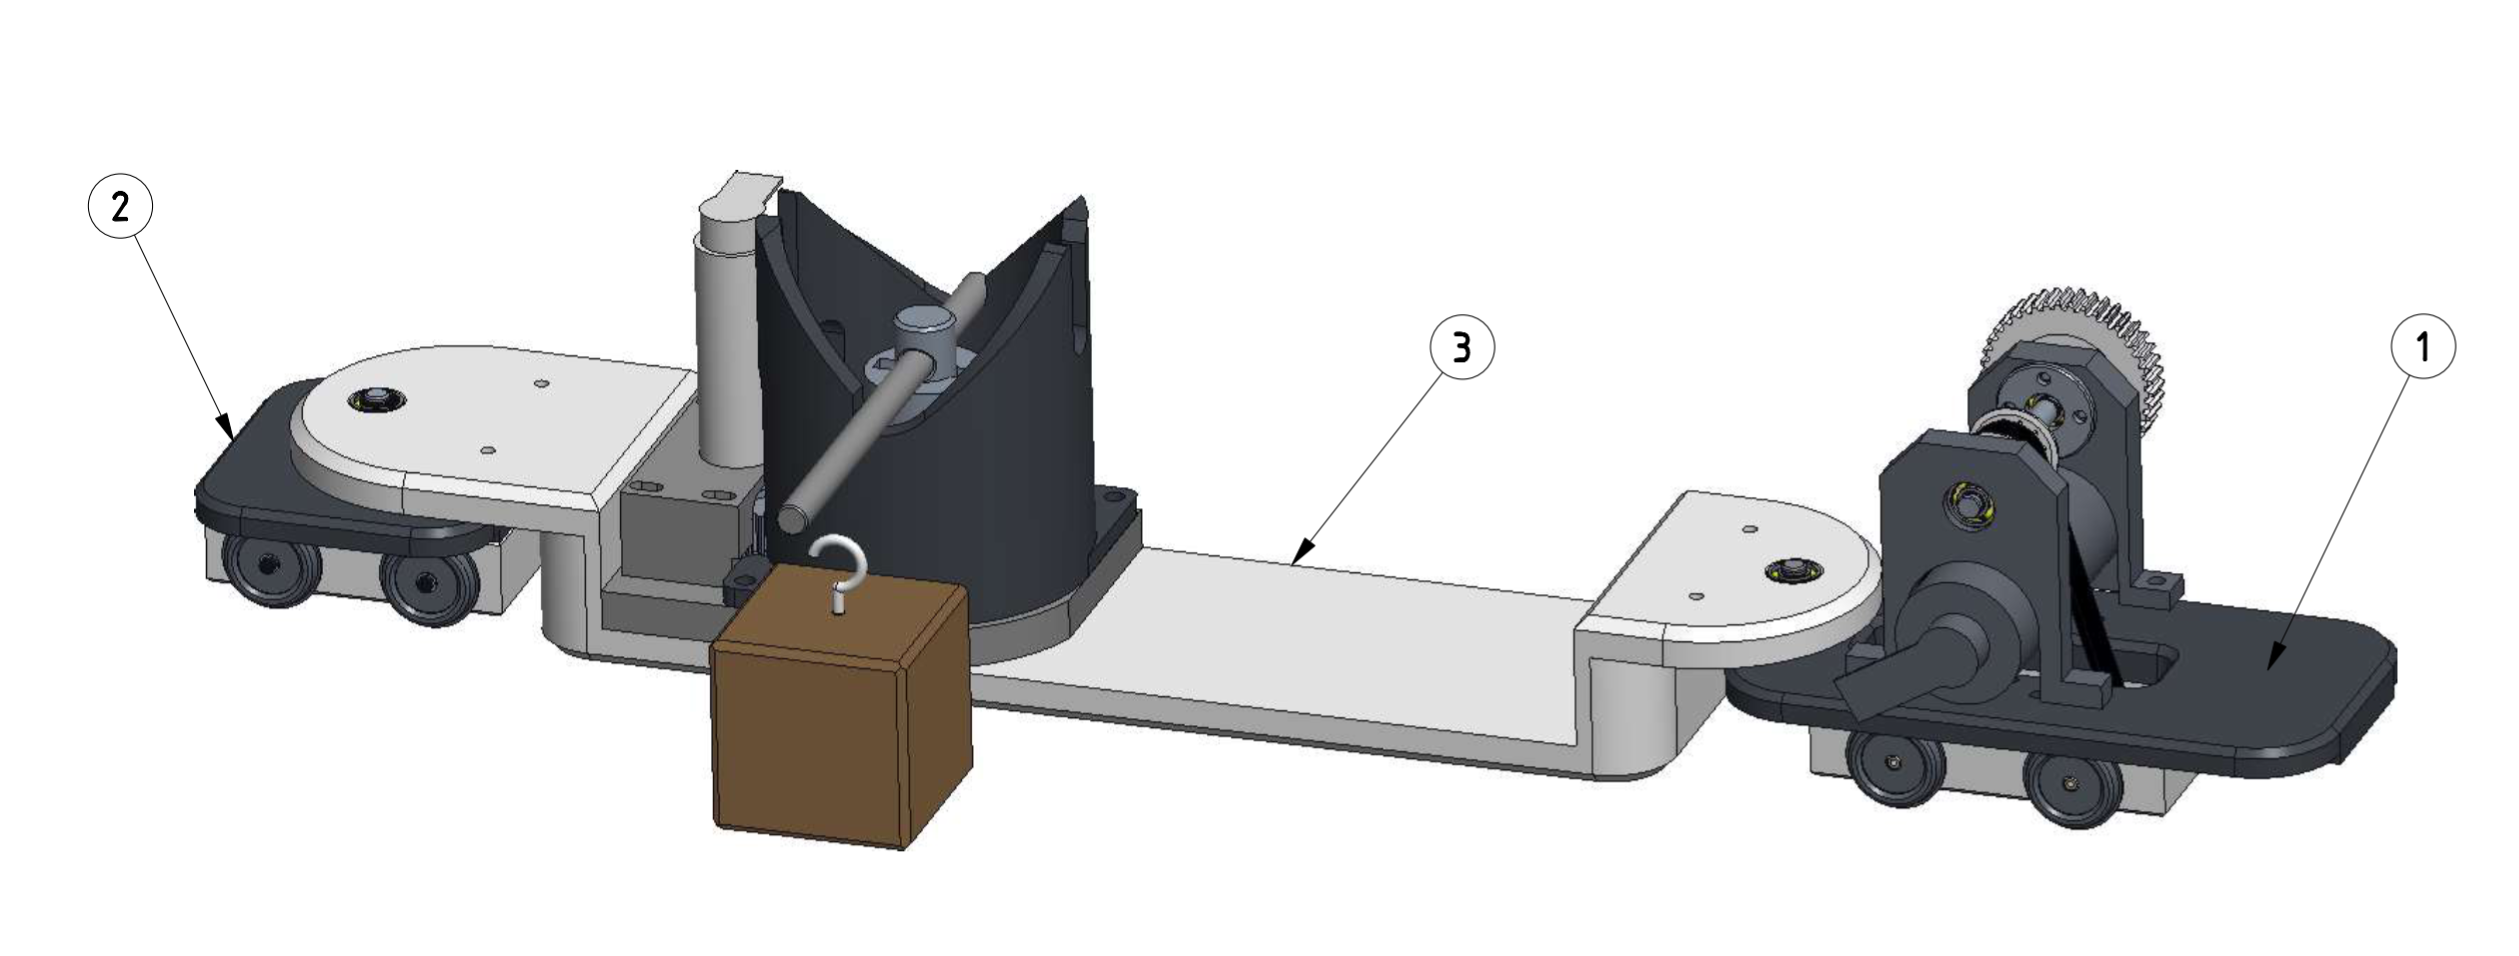
\includegraphics[width=0.9\textwidth]{Lokomotive.png}
        \caption{Baugruppe Lokomotive}
        \label{fig:bg_lokomotive}
    \end{figure}

    \begin{table}[H] \centering
        \begin{tabular}{|l|l|}
        \hline
        \textbf{Position} & \textbf{Bezeichnung}\\
        \hline
        Position 1          & Antriebswagen\\
         \hline
        Position 2          & Führungswagen\\
        \hline
        Position 3          & Ladungsträger\\
        \hline
        Position 4          & Transportgut (Würfel)\\
        \hline
        \end{tabular}

        \caption{Positionsnummern der Lokomotive mit Bezeichnungen}
        \label{tab:bg_lokomotive}
    \end{table}

    In der Querschnittsdarstellung in Abbildung \ref{fig:schnitt_lokomotive} ist die Lagerungen zwischen dem Ladungsträger und dem Antriebswagen beziehungsweise dem Führungswagen besser sichtbar. Ebenfalls sieht man gut, wie der Antriebswagen mit Zahnriemen angetrieben wird. Der Aufbau der Unterbaugruppen wird in den nächsten Abschnitten vorgestellt.\\

    \begin{figure}[H] %Lokomotive im Schnitt
        \centering
        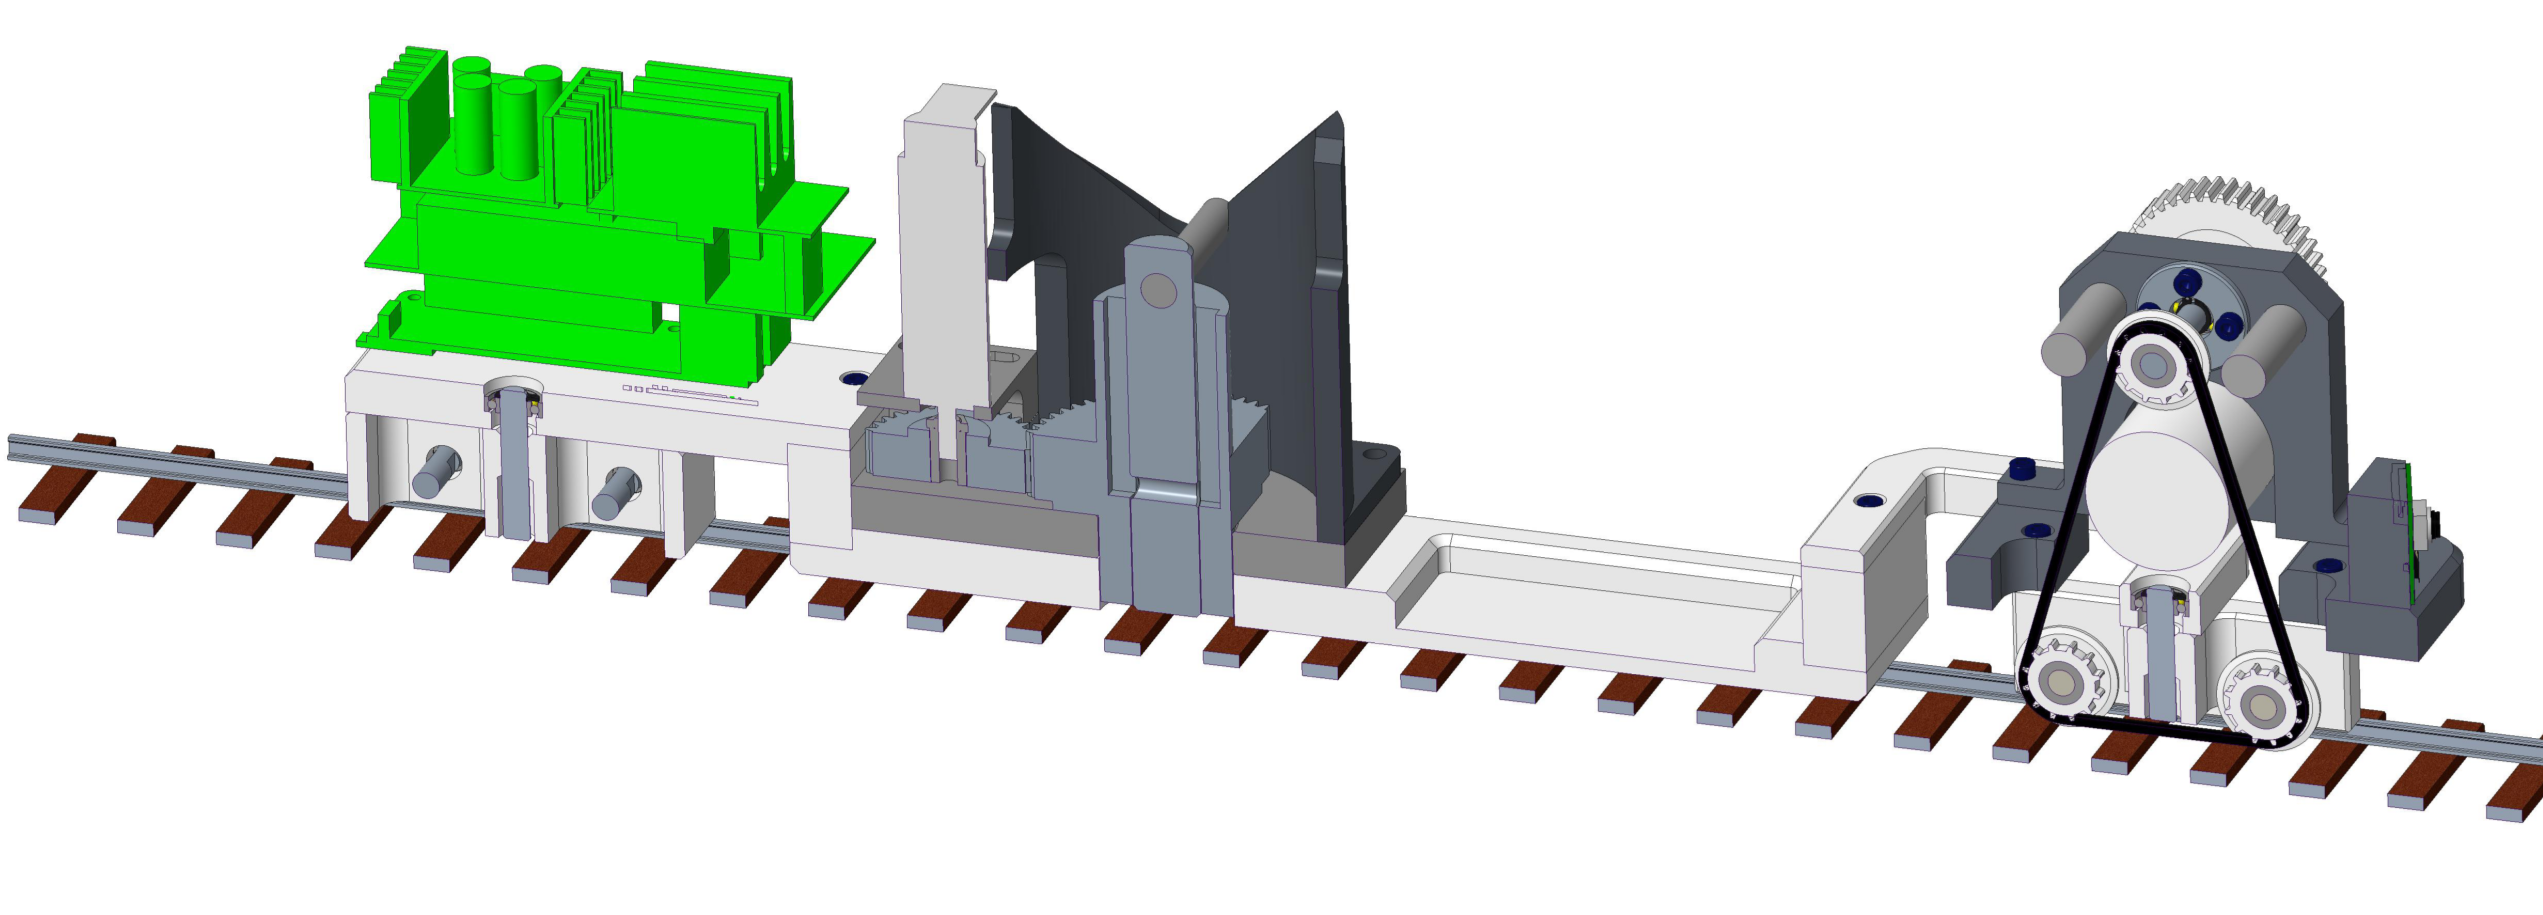
\includegraphics[width=0.7\textwidth]{lokomotive_2.png}
        \caption{Schnittansicht der Lokomotivenbaugruppe}
        \label{fig:schnitt_lokomotive}
    \end{figure}
    \newpage

    \subsubsection{Antriebswagen}
    Der Grundaufbau der beiden Wägen ist derselbe, mit dem Unterschied, dass der Antriebswagen durch einen Motor angetrieben wird. Der Grundwagen beziehungsweise der Führungswagen in Abbildung \ref{fig:expl_fuehrungswagen} (siehe Tabelle \ref{tab:expl_fuehrungswagen}) besteht aus einem Rahmen und einer Platte, welche miteinander verstiftet (Position 2) und verschraubt (Position 3) sind. Im Rahmen werden die beiden Achsen jeweils mit einem Los- (Position 7) und einem Festlager (Position 8) lagert und mit Sicherungsringen (Position 6) gesichert. Die Achsen sind an beiden Enden mit einem Gewinde versehen, damit die Räder bei Bedarf schnell und einfach gewechselt werden können, ohne dass der ganze Wagen auseinander genommen werden muss. Die Anfräsfläche auf der Welle (Position 5) dient für das bessere Befestigen der Räder mit einen Gabelschlüssel.\\

     \begin{figure}[H] %Führungswagen
        \centering
        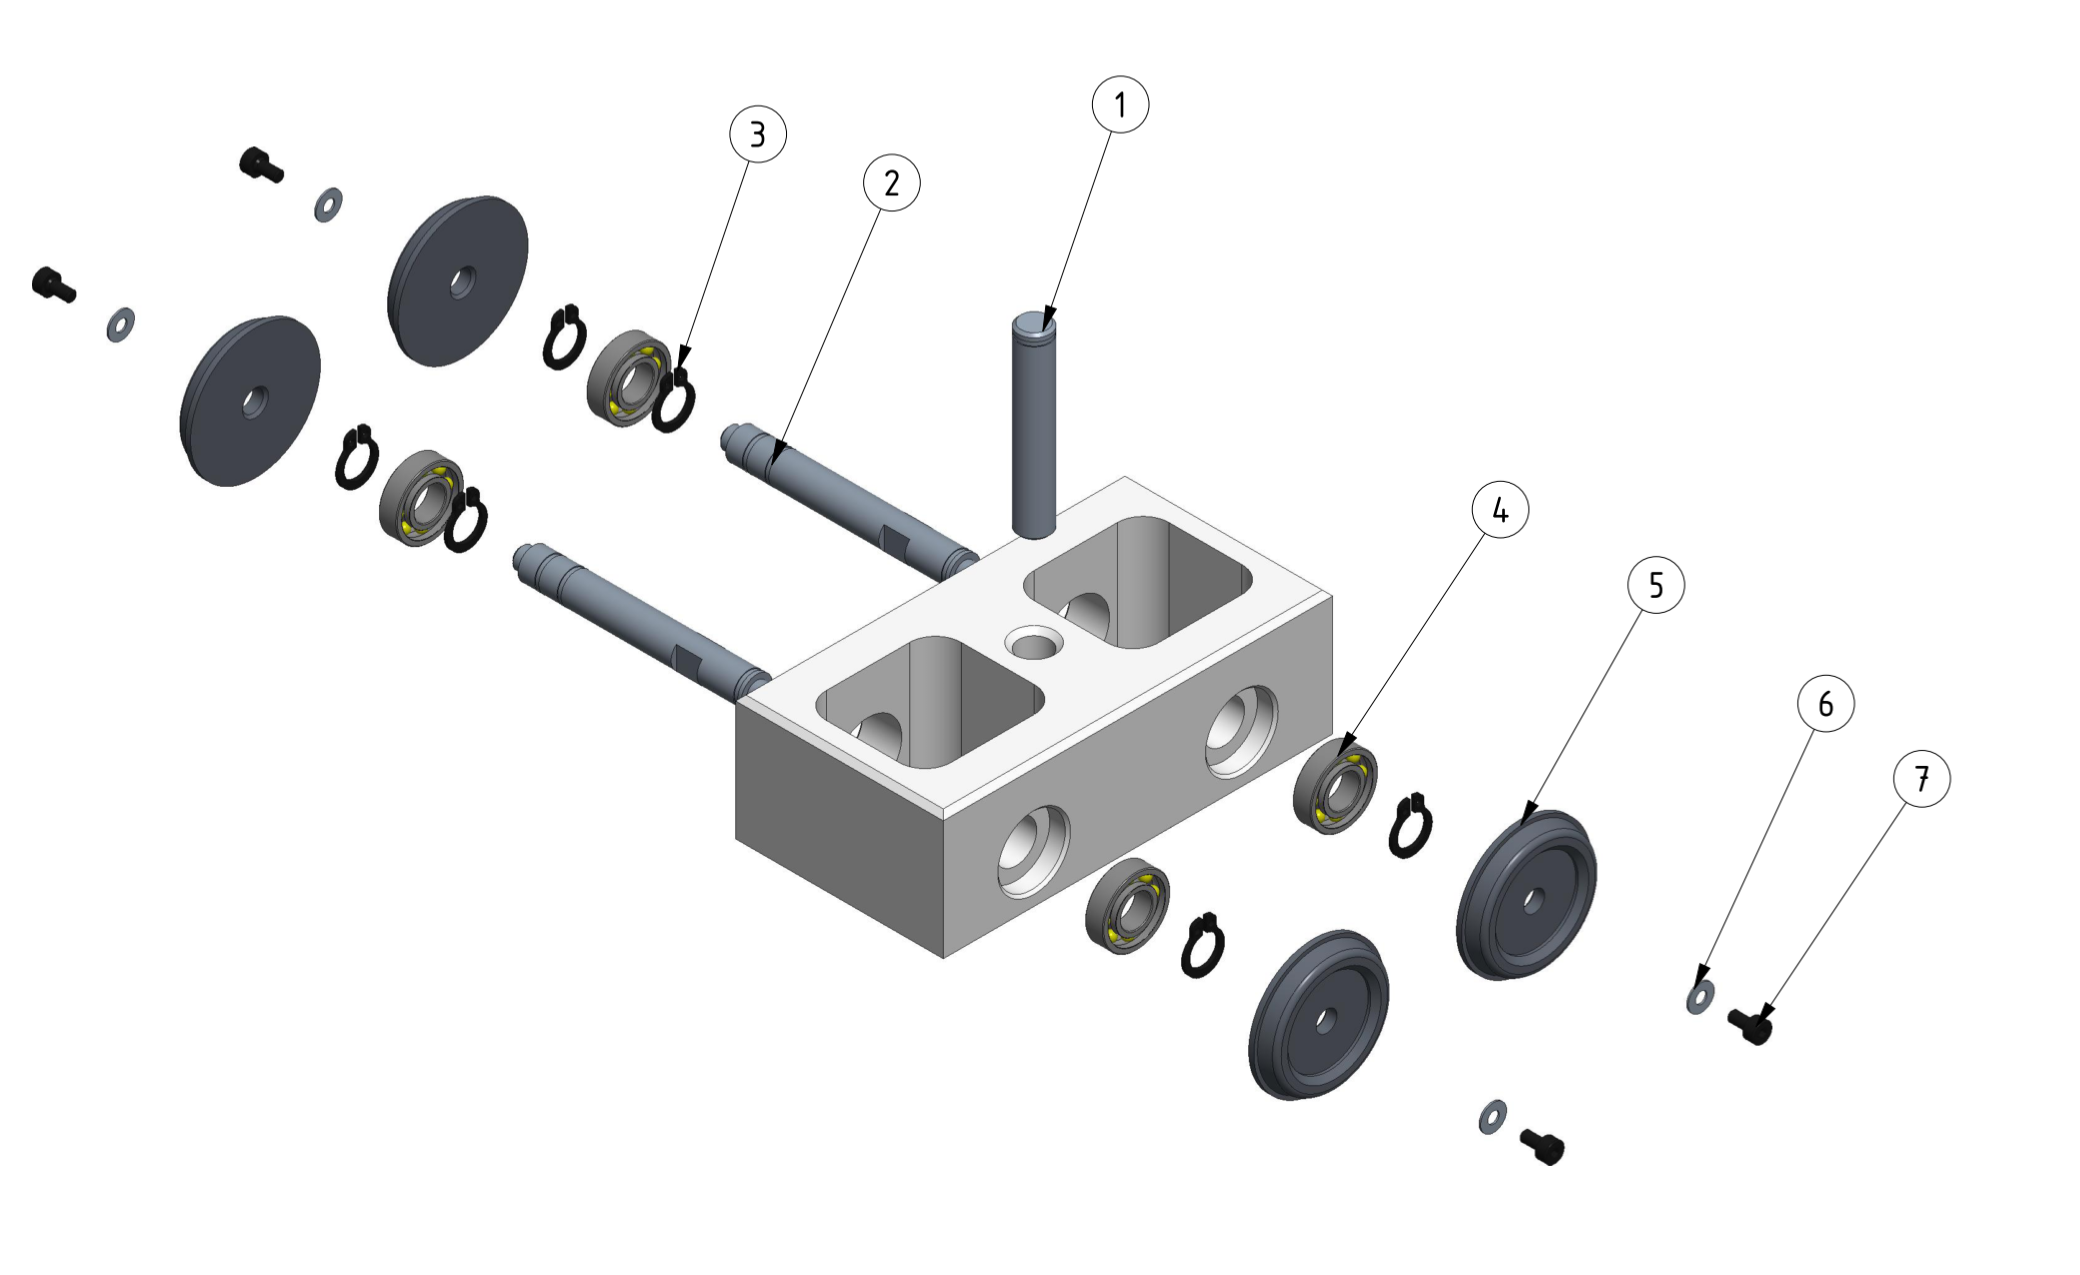
\includegraphics[width=0.9\textwidth]{Fuehrungswagen.png}
        \caption{Explosionsdarstellung Führungswagen}
        \label{fig:expl_fuehrungswagen}
    \end{figure}

    \begin{table}[H] \centering
        \begin{tabular}{|l|l|}
        \hline
        \textbf{Position} & \textbf{Bezeichnung}\\
        \hline
        Position 1          & Drehachse Wagen-Ladungsträger\\
         \hline
        Position 2          & Achsen mit Gewinden an beiden Enden und Anfräsfläche für Gabelschlüssel\\
         \hline
        Position 3          & Sicherungsring für Rillenkugellager\\
        \hline
        Position 4          & Eingepresstes Rillenkugellager (Festlager) bzw. Loslager\\
        \hline
        Position 5          & Rad\\
        \hline
        Position 6          & Unterlagscheibe\\
        \hline
        Position 7          & Zylinderschraube\\
        \hline
        \end{tabular}

        \caption{Explosionsdarstellung Führungswagen}
        \label{tab:expl_fuehrungswagen}
        \end{table}
    \newpage

    Der Antriebswagen in Abbildung \ref{fig:antriebswagen} (siehe Tabelle \ref{tab:expl_antriebswagen}) wie bereits erwähnt grundsätzlich gleich aufgebaut wie der Führungswagen, jedoch ist der Rahmen aufgrund des Riemenantriebs H-Förmig aufgebaut. Das Ziel dieser Konstruktion ist es hauptsächlich den Riemen, falls nötig, schnell wechselbar zu montieren. Durch die H-Form können die Achsen und die Räder für die Riemenmontage am Rahmen montiert gelassen werden. Die Platte, welche am Rahmen angebracht ist, ist für die Kameras für die Signal- und Spurerkennung grösser dimensioniert. Die Kamera für die Spurerkennung wird einstellbar befestigt, damit bei der Testphase des Prototyps Optimierungen des Winkels vorgenommen werden können. Der Stromübetrag von der Schiene auf die Lokomotive erfolgt über vier Schleifkontakte, welche als Einkaufsteile von Lieferanten bezogen werden. Davon sind pro Wagen zwei und jeweils zwischen den Rädern angebracht.\\

    \begin{figure}[H] %Antriebswagen
        \centering
        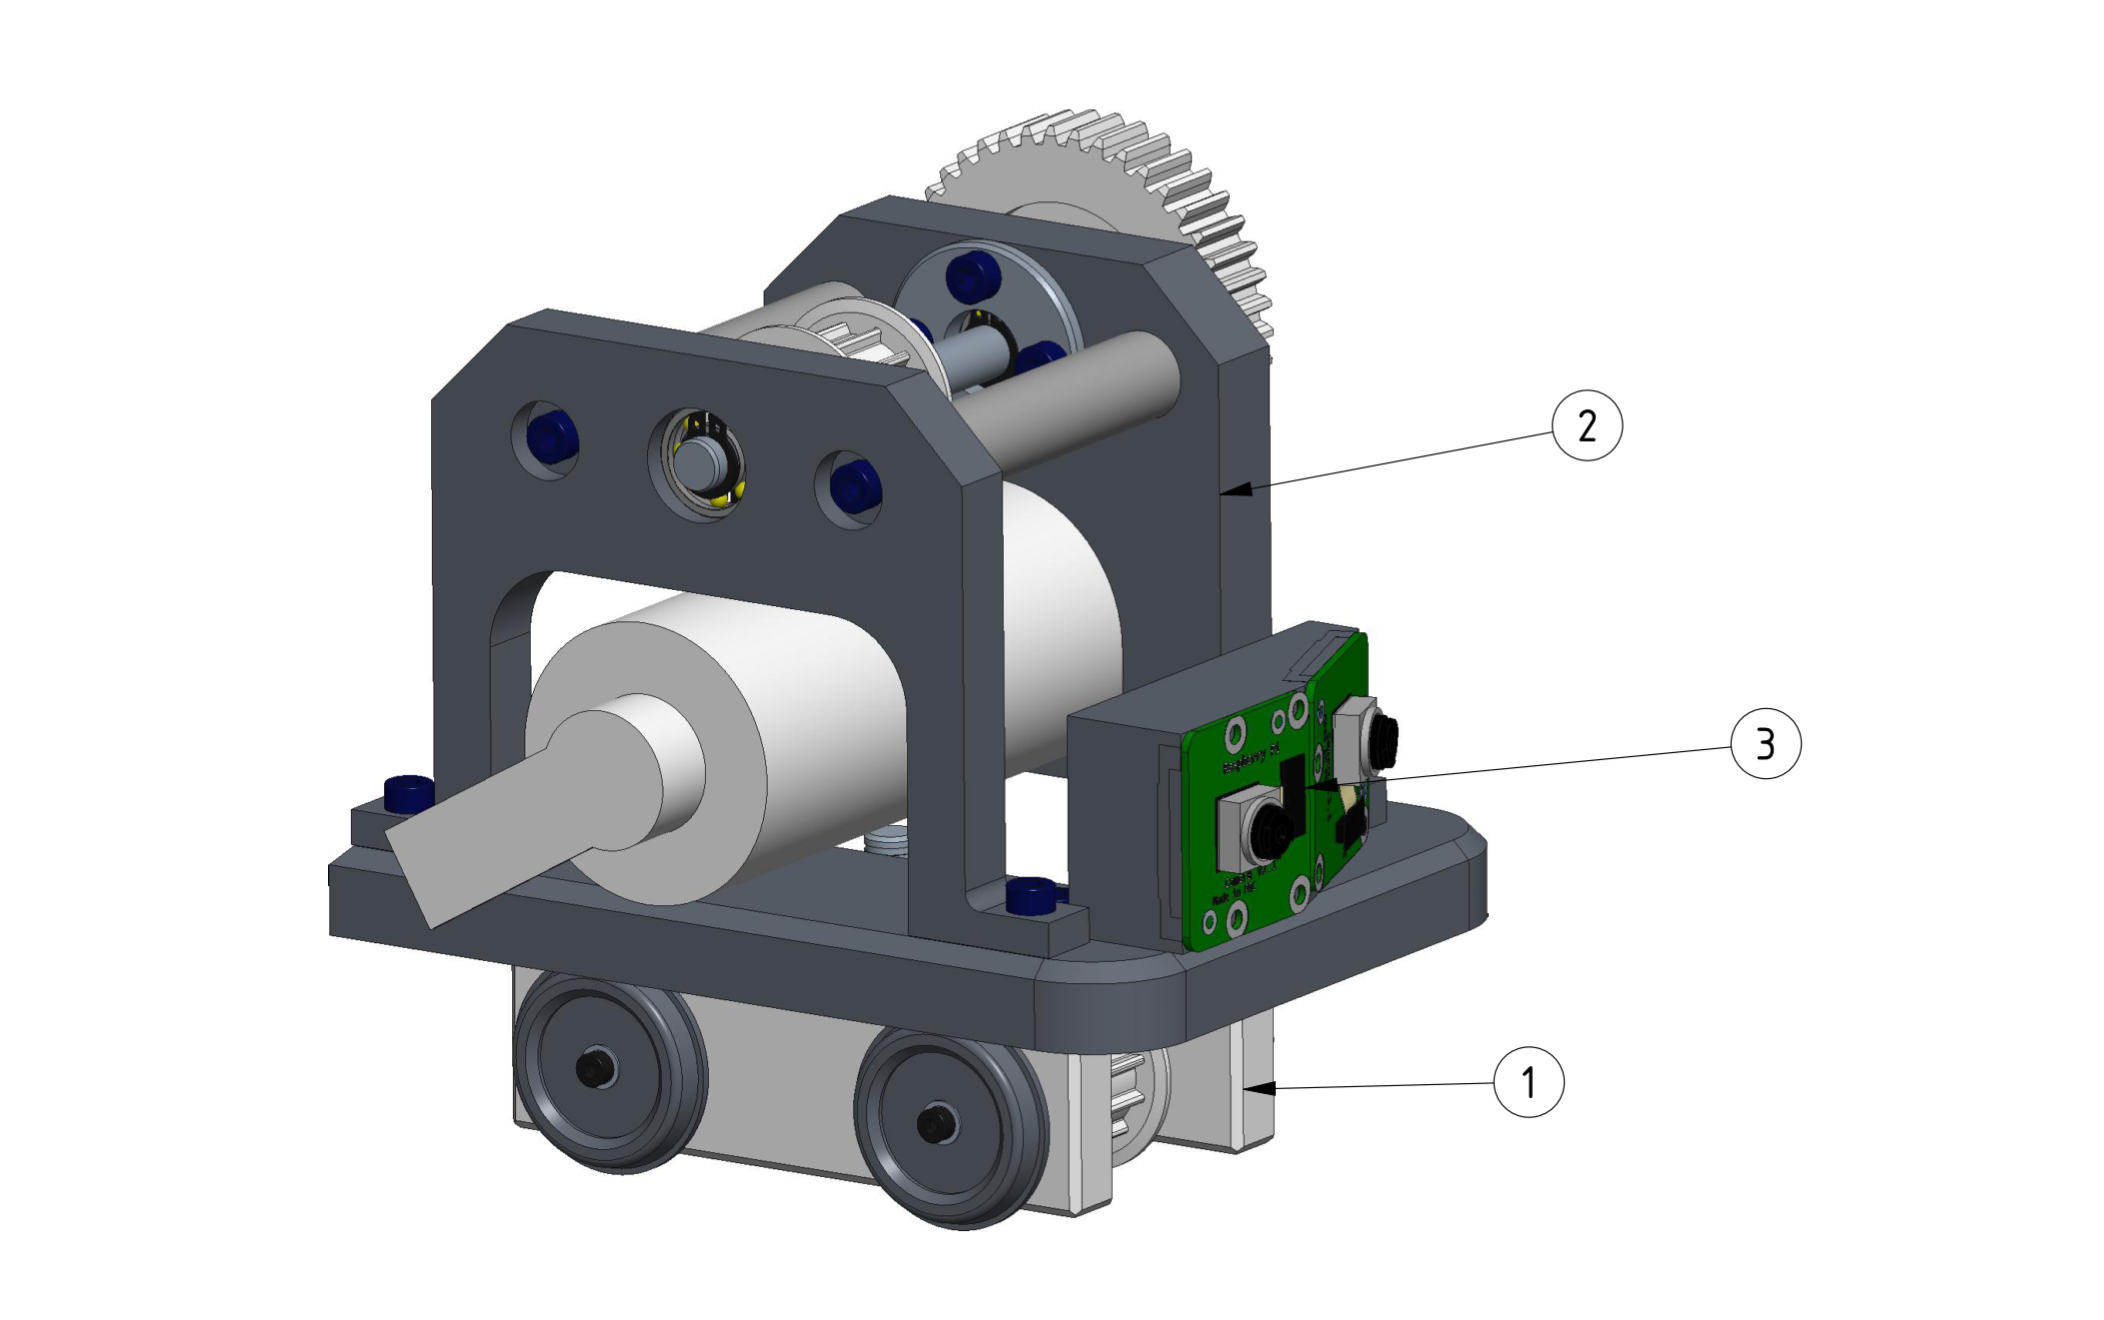
\includegraphics[width=0.9\textwidth]{antriebswagen.png}
        \caption{Baugruppe Antriebswagen}
        \label{fig:antriebswagen}
    \end{figure}

    \begin{table}[H] \centering
        \begin{tabular}{|l|l|}
        \hline
        \textbf{Position} & \textbf{Bezeichnung}\\
        \hline
        Position 1          & Wagen\\
         \hline
        Position 2          & Antriebseinheit\\
        \hline
        Position 3          & Kameras\\
        \hline
    \end{tabular}

    \caption{Explosionsdarstellung Antriebswagen}
    \label{tab:expl_antriebswagen}
    \end{table}

    \newpage

    Die Antriebseinheit in Abbildung \ref{fig:antriebseinheit} (siehe Tabelle \ref{tab:pos_antriebseinheit}) besteht aus einem Grundgestell, an welchem die Lagerung der Antriebswelle und der Motor angebracht sind. Das Drehmoment vom Motor wird über ein geradverzahntes Zahnrad mit einem Übersetzungsverhältnis von 1:2 auf eine Achse übertragen. Von dieser wird es über einen Riemen auf die beiden Radachsen und somit auf die Räder weitergeleitet. Durch die Berechnung der maximalen Geschwindigkeit wird entsprechend der Motor ausgelegt, was im nächsten Abschnitt genauer beschrieben wird.\\

    \begin{figure}[H] %Antriebseinheit
        \centering
        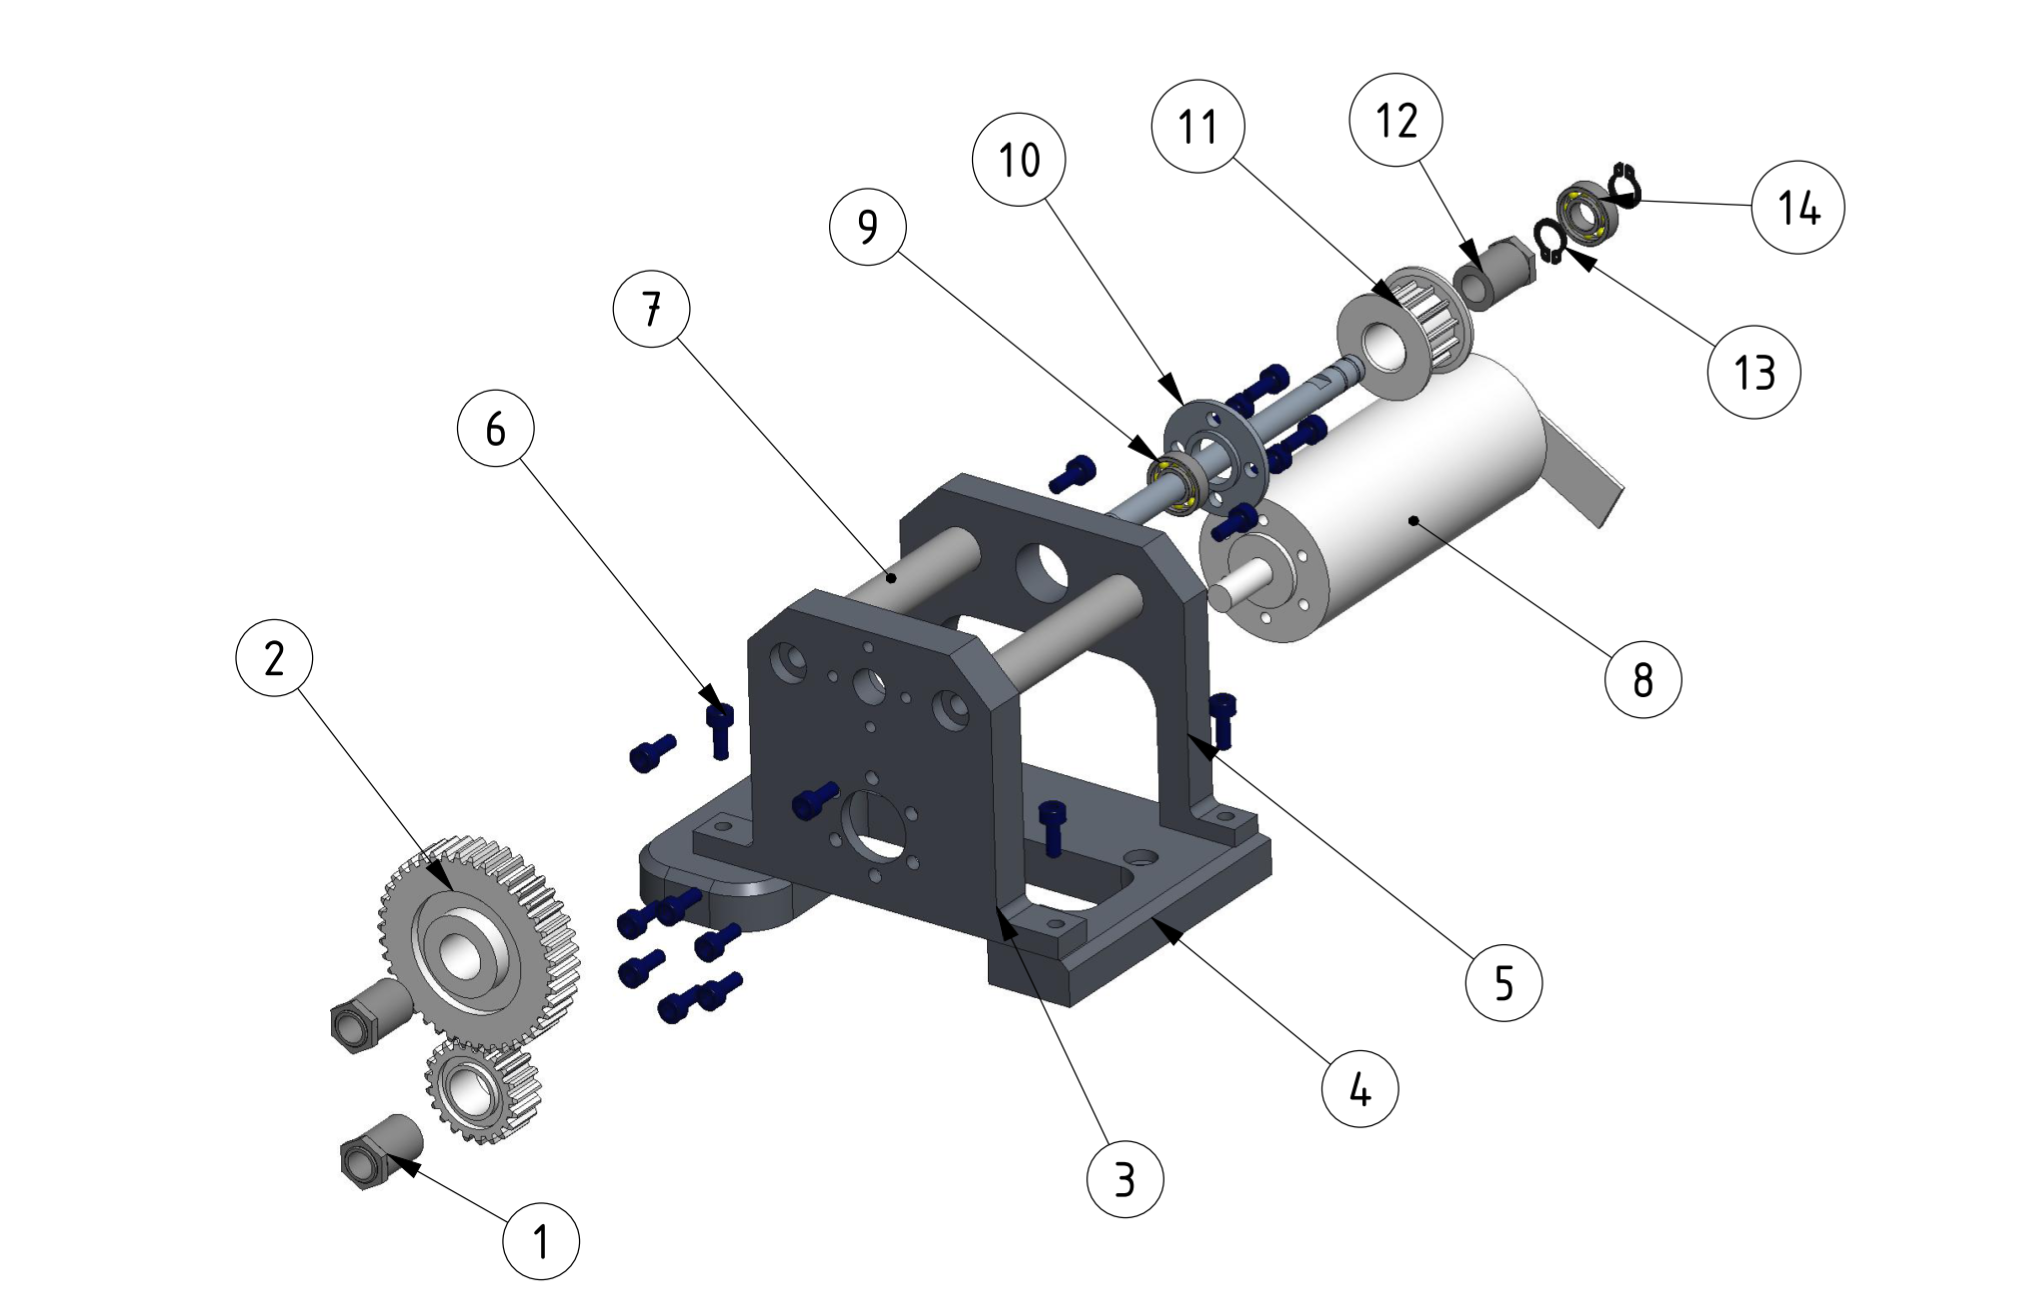
\includegraphics[width=0.9\textwidth]{antriebseinheit.png}
        \caption{Explosionsdarstellung Antriebseinheit}
        \label{fig:antriebseinheit}
    \end{figure}

    \begin{table}[H] \centering
        \begin{tabular}{|l|l|}
        \hline
        \textbf{Position} & \textbf{Bezeichnung}\\
        \hline
        Position 1          & Spannsatz\\
         \hline
        Position 2          & Zahnräder Übersetzung 1:2\\
        \hline
        Position 3          & Motorhalterung\\
        \hline
        Position 4          & Grundplatte\\
        \hline
        Position 5          & Achsenlagerplatte\\
        \hline
        Position 6          & Zylinderschraube\\
        \hline
        Position 7          & Distanzhülsen\\
        \hline
        Position 8          & Motor\\
        \hline
        Position 9          & Rillenkugellager (Loslager)\\
        \hline
        Position 10         & Lagersicherungsplatte\\
        \hline
        Position 11         & Zahnriemenrad\\
        \hline
        Position 12         & Spannsatz\\
        \hline
        Position 13         & Sicherungsring\\
        \hline
        Position 14         & Rillenkugellager (Festlager)\\
        \hline
        \end{tabular}

        \caption{Positionen Antriebseinheit}
        \label{tab:pos_antriebseinheit}
        \end{table}

    \newpage

    \textbf{Beschleunigungsberechnung}\\
    Wie schnell die Lokomotive beschleunigen kann hängt von der Reibung zwischen Rad und schiene und der Masse des Zuges ab. Die Grunddefinition der Beschleunigung ist der Quotient von Kraft und Masse. Die Reibung ist durch den Reibkoeffizienten bestimmt, welcher sich von Materialpaarung zu Materialpaarung unterscheidet. Zusätzlich ist der Reibkoeffizient von der Oberflächenbeschaffenheit, der Rauigkeit, abhängig. Je die Rauigkeit, desto mehr Reibung entsteht und desto schneller kann beschleunigt werde. Die Kraft, um das Fahrzeug aus dem Stillstand zu beschleunigen ist grösser, als wenn es bei einer gewissen Geschwindigkeit weiter beschleunigt wird. Dies ist auf Grund des Trägheitsmomentes des Zuges. \\

    \begin{table}[H] \centering
        \begin{tabular}{|l|l|l|}
        \hline
        \textbf{Material Schiene} & \textbf{Material Rad} & \textbf{Reibungskoeffizient}\\
        \hline
        Stahl                                & Stahl        & 0.05\\
        \hline
        Stahl                                & Holz         & 0.12\\
        \hline
        Stahl                                & Kunststoff   & 0.08\\
        \hline
        Stahl                                & Gummi        & 0.3\\
        \hline
        \end{tabular}

        \caption{Reibungskoeffizienten verschiedener Materialpaarungen}
        \label{tab:com_tiny_pi}
        \end{table}

    Um die maximale Beschleunigung zu berechnen, wird das Gesamtgewicht der Lokomotive auf die vier Räder aufgeteilt. In der Tabelle \ref{tab:groessen_beschleunigung} sind die gegeben Grössen für die nachfolgenden Berechnungen aufgelistet.\\

    \begin{table}[H] \centering
        \begin{tabular}{|l|l|}
        \hline
        \textbf{Grösse} & \textbf{Wert}\\
        \hline
        Durchmesser Rad [D]          & 30 Milimeter\\
         \hline
        Reibungskoeffizient [k]      & 0.3\\
        \hline
        \end{tabular}

        \caption{Grössen für die Beschleunigungsberechnung}
        \label{tab:groessen_beschleunigung}
        \end{table}

    F\textsubscript{Rad}=\(\frac{F\textsubscript{G}}{8}\)=\(\frac{m*g=3kg*9.81m/s^2}{8}\)=0.375N\\

    F\textsubscript{Reibung}=\(F\textsubscript{Rad}*k\)=\(0.375N*0.3=29.4N\)=0.1125N\\

    M\textsubscript{Rad}=\(F\textsubscript{Rad}*2*D\textsubscript{Rad}\)=\(\frac{m*g=3kg*9.81m/s^2}{8}\)=0.375Nm\\

    a\textsubscript{max}=\(\frac{F\textsubscript{Reibung}}{\frac{F\textsubscript{Rad}}{g}}\)=\(\frac{0.1125N}{\frac{0.375N}{9.81m/s^2}}=2.94m/s^2\)\\

    \label{GeschwindigkeitsberechnungFahrwerk}
    \textbf{Geschwindigkeitsberechnung}\\
    Die Fahrgeschwindigkeit der Lokomotive wird durch zwei Faktoren bestimmt. Einerseits muss die maximale Geschwindigkeit der Anforderungsliste eingehalten werden und andererseits wird die Geschwindigkeit in der Kurvenfahrt durch den Schwerpunkt des Fahrzeuges eingeschränkt. Nachdem die Lokomotive auf die Fahrtgeschwindigkeit beschleungigt wurde, ist die Rollreibung das einzige, was der Motor mit seiner Leistung kompensieren muss.\\

    In der Anforderungsliste wurde eine minimale Geschwindigkeit von 0.5 Meter pro Sekunde festgelegt. Der begrenzende Faktor der Geschwindigkeit in der Kurve ist der Schwerpunkt der Lokomotive. Je tiefer dieser ist, umso schneller kann die Kurve abgefahren werden. Über die Zentripedalkraft und die Gewichtskraft der Lokomotive wird die Momentengleichung aufgestellt und Anhand der gegebeen Werten in Tabelle \ref{tab:geschwindigkeitsberechnung} wird die maximal erreichbare Geschwindigkeit in der Kurve, ohne aus den Gleisen zu kippen, berechnet.\\

    Das Kippmoment wird durch den Aufbau der Lokomotive minimiert. Da der Schwerpunkt durch die beiden Wagen mehr in das Zentrum des Kreismittelpunktes rückt.\\

    \begin{table}[H] \centering
        \begin{tabular}{|l|l|}
        \hline
        \textbf{Grösse} & \textbf{Wert}\\
        \hline
        Minimaler Radius  [r]                               & 0.8 Meter\\
         \hline
        Masse [m]                                           & 3 Kilogramm\\
        \hline
        Schwerpunkt in x-Achse (maximaler Wert) [x]         & 0.025 Meter\\
        \hline
        Schwerpunkt in y-Achse (maximaler Wert) [y]         & 0.08 Meter\\
        \hline
        \end{tabular}

        \caption{Grössen für die Geschwindigkeitsberechnung}
        \label{tab:geschwindigkeitsberechnung}
        \end{table}

    Die Gewichts- und Zentripedalkraft, welche das Gleichungssystem bilden, sind wie folgt definiert:\\

    F\textsubscript{G}=\(m*g=3kg*9.81m/s^2=29.4N\)\\

    F\textsubscript{max z}=\(\frac{m*v^2}{r}\)=\(\frac{3kg*(1.28m/s)^2}{0.8}\)\\

    Da das Drehmoment eine vektorielle Grösse ist, müssen die beiden entstehenden Momente am Drehpunkt "P" am Gleis zusammen Null ergeben. Oder anderst gesagt müssen die beiden Momente gleich gross sein, damit das System "statisch" bestimmt ist. Die Berechnungen sind auf den kleinsten Kurvenradius ausgelegt, da dort die grössere Zentripedalkraft entsteht. Nun werden die ob\\

    F\textsubscript{max z}=\(\frac{F\textsubscript{G}*x}{y}\)=\(\frac{29.4N*0.025m+9.2N*a}{0.08m}\)=9.2N\\

    \subsubsection{Ladungsträger}
    Der Ladungsträger ist das Verbindungselement von Antriebswagen und Führungswagen. Er wird an beiden Enden drehbar mit je einem Radial- und Axialkugelager gelagert. Der Träger besteht aus drei Teilen (siehe Abbidlung \ref{fig:expl_ladungstraeger}). Der Hauptgrund ist die einfachere, materialsparende sowie kostengünstigere Herstellung. Andererseits muss der Träger \\

    %Berechnung Kugellagerkräfte Radial wie auch Axial

    \begin{figure}[H] %Ladungsträger
        \centering
        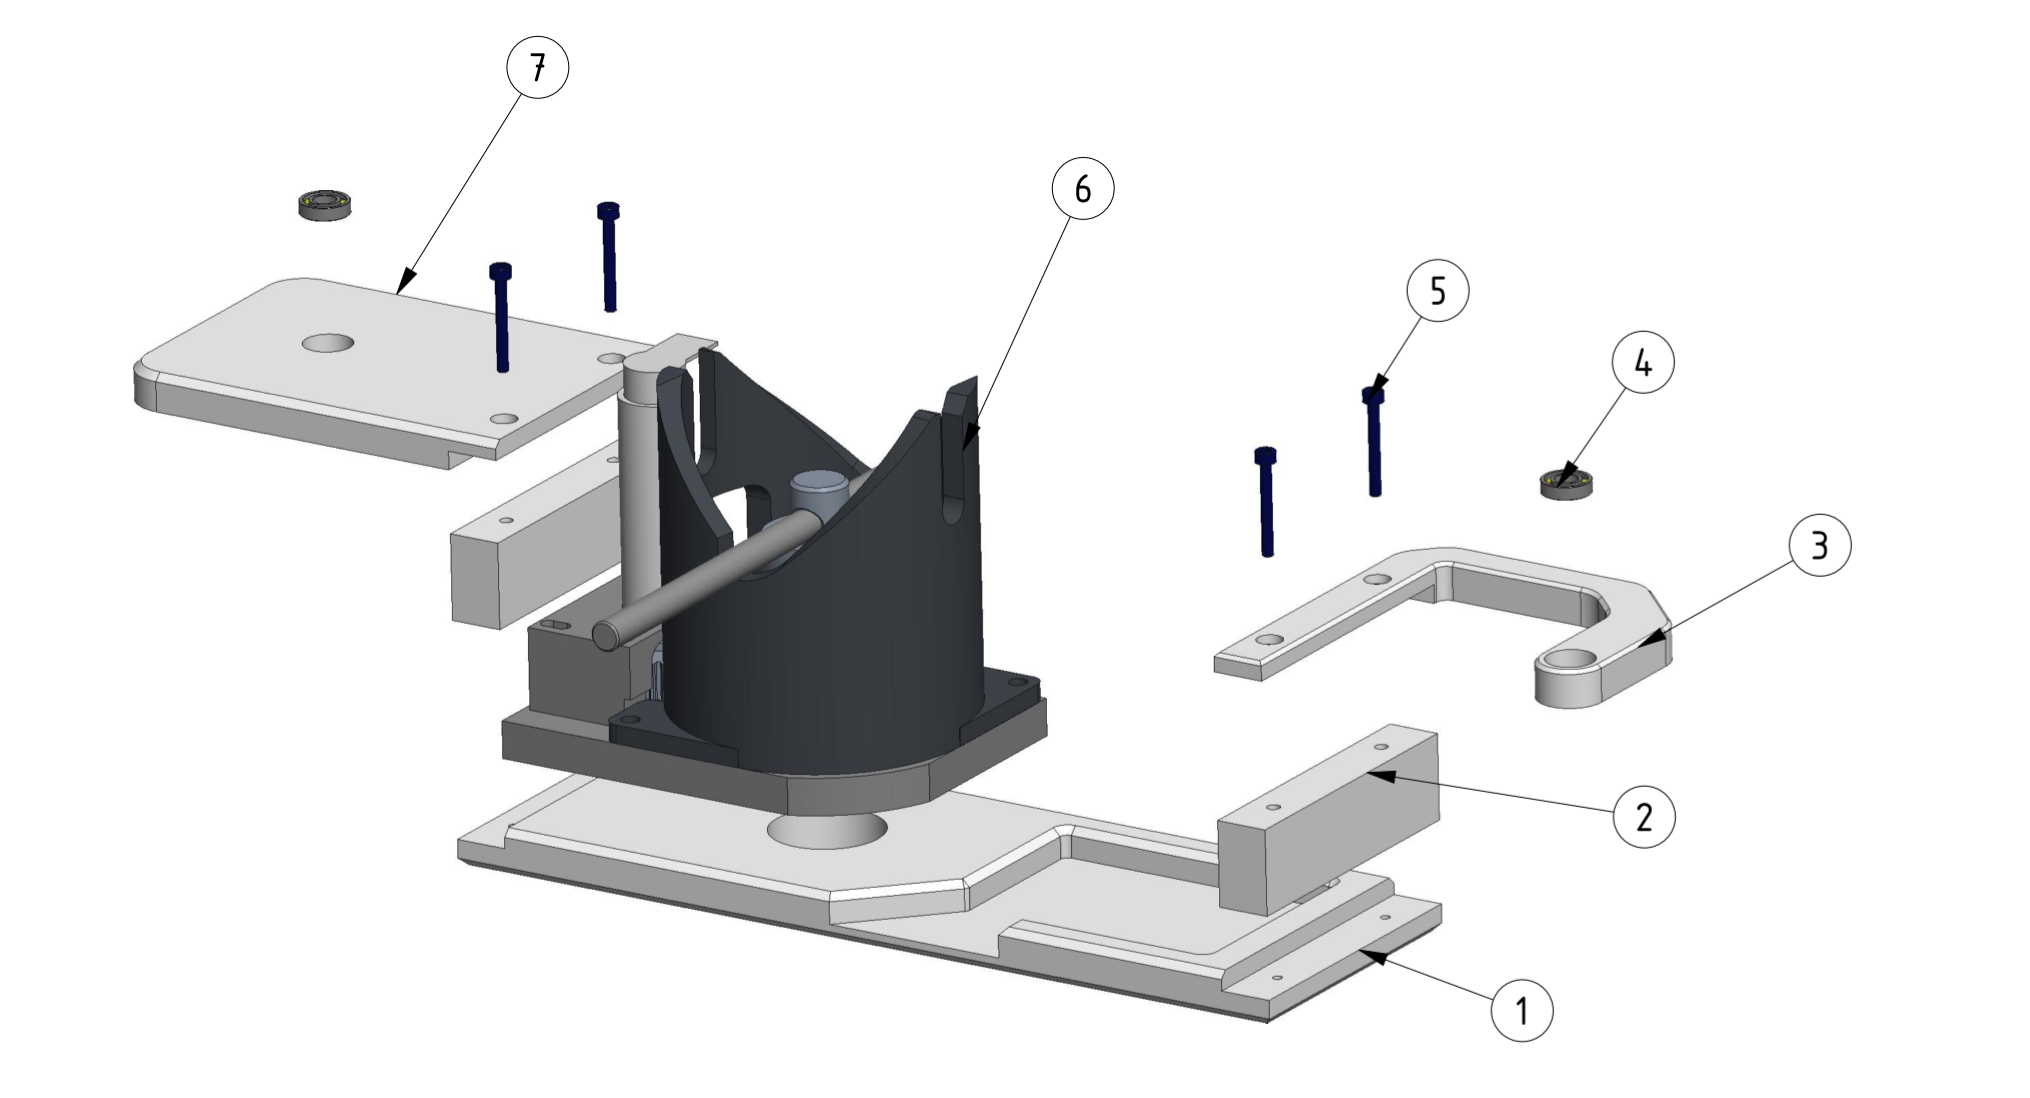
\includegraphics[width=0.9\textwidth]{ladungstraeger.png}
        \caption{Explosionsdarstellung Ladungsträger}
        \label{fig:expl_ladungstraeger}
    \end{figure}

    \begin{table}[H] \centering
        \begin{tabular}{|l|l|}
        \hline
        \textbf{Position} & \textbf{Bezeichnung}\\
        \hline
        Position 1          & Grundplatte\\
         \hline
        Position 2          & Zwischenplatte\\
        \hline
        Position 3          & Bügelgelenk\\
        \hline
        Position 4          & Rillenkugellager\\
        \hline
        Position 5          & Zylinderschrauben\\
        \hline
        Position 6          & Würfelkran\\
        \hline
        Position 7          & Plattengelenk\\
        \hline
        \end{tabular}

        \caption{Positionen des Ladungsträgers}
        \label{tab:pos_ladungstraeger}
        \end{table}

\end{document}